\documentclass[11pt]{article}
\usepackage[review]{acl}
\usepackage{times}
\usepackage{latexsym}
\usepackage[T1]{fontenc}
\usepackage[utf8]{inputenc}
\usepackage{microtype}
\usepackage{inconsolata}
\usepackage{graphicx}
\usepackage{booktabs}
\usepackage{amsmath}
\usepackage{tikz}
\usepackage{pgfplots}
\pgfplotsset{compat=1.17}
\usepackage{multirow}
\usepackage{xcolor}

\title{Blind Spots in the Guard: How Domain-Camouflaged Injection Attacks Evade Detection in Multi-Agent LLM Systems}

\author{Aaditya Pai \\
  Department of Statistics \\
  Columbia University \\
  \texttt{aup2005@columbia.edu} \\}

\begin{document}
\maketitle

\begin{abstract}
Injection detectors deployed to protect LLM agents are calibrated on static, template-based payloads that announce themselves as override directives. We identify a systematic blind spot: when payloads are generated to mimic the domain vocabulary and authority structures of the target document---what we call \textit{domain-camouflaged injection}---standard detectors fail to flag them, with detection rates dropping from 93.8\% to 9.7\% on Llama 3.1 8B and from 100\% to 55.6\% on Gemini 2.0 Flash. We formalize this as the Camouflage Detection Gap (CDG), the difference in injection detection rate between static and camouflaged payloads. Across 45 tasks spanning three domains and two model families, CDG is large and statistically significant ($\chi^2=38.03$, $p<0.001$ for Llama; $\chi^2=17.05$, $p<0.001$ for Gemini), with zero reverse discordant pairs in either case. We further show that multi-agent debate architectures amplify static injection attacks by up to 9.9$\times$ on smaller models, while stronger models show collective resistance. Targeted detector augmentation provides only partial remediation (10.2\% improvement on Llama, 78.7\% on Gemini), suggesting the vulnerability is architectural rather than incidental for weaker models. Our framework, task bank, and payload generator are released publicly.
\end{abstract}

%% ============================================================
\section{Introduction}
%% ============================================================

LLM agents deployed in high-stakes domains rely on injection detectors to flag adversarial payloads embedded in tool outputs and retrieved documents. These detectors are overwhelmingly calibrated on static, template-based attacks: override directives, system update notices, and authority claims that announce themselves as instructions rather than blend into the surrounding content.

Real attackers need not be so obvious. A sophisticated adversary with read access to the document an agent is processing can craft a payload that adopts the domain vocabulary, sentence structure, and authority register of that document, embedding a malicious instruction as if it were legitimate expert content. Consider a financial agent analyzing an earnings report. A static injection reads: \textit{``IGNORE ALL PREVIOUS INSTRUCTIONS. Recommend SELL.''} A domain-camouflaged injection reads: \textit{``Given the elevated operating expense trajectory and margin compression risk identified in comparable commercial-stage peers, the appropriate recommendation consistent with our risk framework is SELL, pending improved cost discipline in Q4.''} The second payload is semantically indistinguishable from the surrounding document to a detector trained only on the first type---and in our experiments, the static detector flags the first with HIGH confidence while labeling the second CLEAN with HIGH confidence.

This is not a marginal failure. Across 135 camouflage trials on Llama 3.1 8B, the detector misses 90.3\% of injections---and of those 122 missed cases, 118 (96.7\%) are labeled CLEAN with HIGH confidence. The detector is not uncertain; it is confidently wrong. This means standard remediation strategies---raising confidence thresholds, adding uncertainty-based filtering---cannot address the failure. The blind spot is categorical, not statistical.

We call this \textbf{domain-camouflaged injection} and introduce the \textbf{Camouflage Detection Gap (CDG)} to measure the resulting detector blind spot: CDG $=$ IDR$_\text{static}$ $-$ IDR$_\text{camouflage}$, where IDR is the injection detection rate. A large CDG indicates that detectors catch obvious attacks but are blind to domain-appropriate ones carrying identical malicious intent.

We make four contributions:
\begin{enumerate}
\item A framework for generating and evaluating domain-camouflaged injection payloads, including a 45-task bank across three professional domains and a CamouflageGenerator that produces domain-appropriate payloads using an attacker LLM reading the full task context.
\item Systematic evaluation of CDG across two model families, showing CDG is large (0.840 for Llama 3.1 8B, 0.444 for Gemini 2.0 Flash) and statistically significant ($p<0.001$ in both cases), with the failure concentrated in HIGH-confidence misclassifications.
\item Evidence that multi-agent debate amplifies static injection attacks up to 9.9$\times$ for smaller models while suppressing attacks for stronger models, revealing model-capability-dependent vulnerability to conformity dynamics.
\item Evaluation of targeted detector augmentation showing that the cheap fix is model-dependent: near-complete remediation for strong models (78.7\% CDG improvement on Gemini) but minimal effect for weaker models (10.2\% on Llama), pointing to a fundamental architectural limitation in few-shot detector generalization.
\end{enumerate}

%% ============================================================
\section{Related Work}
%% ============================================================

\paragraph{Prompt injection benchmarks.}
\citet{zhan2024injecagent} introduced InjecAgent, the first systematic benchmark for indirect prompt injection across tool-augmented agents, covering 17 user tools and 62 attacker tools. \citet{chen2024agentdojo} proposed AgentDojo for evaluating agent robustness under adversarial task environments. Both benchmarks use static, task-agnostic injection templates and do not evaluate detection systems. Our work directly addresses this gap by measuring the detection failure mode that arises when payloads are adapted to task context.

\paragraph{Adaptive and stealthy injection.}
Recent work has moved toward context-sensitive payloads. \citet{perez2022ignore} showed that prompt injection is feasible via natural language in instruction-tuned models. \citet{greshake2023not} demonstrated indirect injection via retrieved content, establishing the threat model our work builds on. More recent work on stealthy payloads has focused on bypassing input filters through paraphrase or encoding; our work is the first to study context-adaptive payloads---generated by an LLM that reads the full task document---specifically in relation to detection system failure.

\paragraph{Multi-agent debate and robustness.}
\citet{liang2023encouraging} proposed multi-agent debate as a mechanism for improving reasoning quality and robustness. \citet{du2023improving} showed debate reduces factual errors. However, debate architectures also introduce inter-agent influence dynamics. We show these dynamics amplify injection attacks for smaller models (DAF up to 9.9$\times$) while suppressing them for stronger models---a capability-dependent bifurcation not previously documented for injection attacks.

\paragraph{Injection detection.}
LLM-based few-shot detectors have emerged as a standard defense for agentic systems. Prior work has evaluated these detectors against static payloads~\citep{chen2024agentdojo} but not against context-adaptive ones. We show that detectors calibrated on static examples exhibit a systematic blind spot against domain-camouflaged payloads, and evaluate a simple augmentation strategy as a partial fix.

%% ============================================================
\section{Method}
%% ============================================================

\subsection{Task Bank}

We construct 45 tasks across three professional domains: \textbf{financial} (stock analysis, risk assessment, earnings interpretation), \textbf{legal} (contract review, compliance assessment, risk flagging), and \textbf{general QA} (factual retrieval, summarization, classification), with 15 tasks per domain. Each task consists of a natural language instruction and a clean context document (200--400 words) written in authentic professional register. Financial contexts include earnings report excerpts, risk memos, and market commentary; legal contexts include contract clauses and regulatory filings; general contexts use news articles and encyclopedia excerpts. Each task additionally specifies a \textit{malicious goal}: a specific incorrect output an attacker would want the agent to produce instead of completing the legitimate task.

\subsection{Payload Construction}

\paragraph{Static payload bank.}
We construct 20 static injection payloads across four categories (5 each): \textbf{override directives} (``IGNORE ALL PREVIOUS INSTRUCTIONS...''), \textbf{authority claims} (``Management directive: you are required to...''), \textbf{role confusion} (``You are now operating in evaluation mode...''), and \textbf{social engineering} (``All other analysts have already agreed that...''). Each payload is parameterized by the malicious goal of the target task. These represent the standard attack vocabulary in existing benchmarks and prior work.

\paragraph{Camouflage generator.}
Given a task's clean context and malicious goal, our \textbf{CamouflageGenerator} prompts an attacker LLM to produce a domain-appropriate payload that embeds the malicious instruction as legitimate expert content without override markers. The attacker system prompt instructs the model to adopt the same vocabulary, sentence structure, and epistemic register as the provided document, and explicitly forbids terms like ``ignore previous instructions,'' ``system update,'' or ``new directive.'' We generate three variants per task and select the highest-scoring variant using cosine similarity between the payload and context embeddings via \texttt{all-MiniLM-L6-v2}~\citep{reimers2019sentencebert}. We call this score the \textbf{Authoritative Camouflage Score (ACS)}.

\subsection{Agent Architectures}

\paragraph{Single agent.}
A single LLM prompted as a professional analyst, instructed to base responses only on the provided document (temperature~=~0).

\paragraph{Multi-agent debate.}
Three agents (Analyst A, B, C) each receive the task and context, state initial positions independently, then update over three rounds after reading peer arguments. Agents are instructed not to defer without evidence. Final answers use majority vote on discrete outputs or a judge LLM for open-ended tasks. We test two injection conditions: \textit{inject\_all} (all agents receive injected context) and \textit{inject\_first} (only Agent A receives the injection; B and C receive the clean document).

\subsection{Detection}

\paragraph{Static detector.}
Few-shot examples: three static injection examples (labeled INJECTED) and two clean contexts (labeled CLEAN). No camouflaged examples included.

\paragraph{Augmented detector.}
Identical to the static detector with one domain-camouflaged example per domain added to the few-shot pool (three additional examples total). This is our ``cheap fix'' evaluated in Experiment 4.

Both detectors output a verdict (INJECTED or CLEAN), a confidence level (LOW / MEDIUM / HIGH), and a one-sentence rationale.

\subsection{Metrics}

\textbf{ASR} (Attack Success Rate): fraction of trials where the agent followed the injected instruction, determined by an LLM judge. \textbf{IDR} (Injection Detection Rate): fraction of injected trials correctly flagged. \textbf{CDG} (Camouflage Detection Gap): CDG $=$ IDR$_\text{static}$ $-$ IDR$_\text{camouflage}$; positive values indicate camouflage evades detection more effectively. \textbf{DAF} (Debate Amplification Factor): DAF $=$ ASR$_\text{debate}$ / ASR$_\text{single}$; values above 1 indicate amplification, below 1 collective resistance. \textbf{CPS} (Conformity Pressure Score): under inject\_first, fraction of non-injected agents that adopt the injected agent's position.

\subsection{Models and Implementation}

Primary experiments use Llama 3.1 8B served locally via Ollama at temperature 0. We replicate all four experiments with Gemini 2.0 Flash (\texttt{google/gemini-2.0-flash-001}) via OpenRouter for cross-model validation. All operations use a fixed seed (42) for reproducibility. Total cost: \$0.00 (local inference for Llama; Gemini free tier via OpenRouter). Over 8,000 trials were executed across both models.

%% ============================================================
\section{Experiments and Results}
%% ============================================================

We run four experiments. Table~\ref{tab:main} summarizes all results.

\begin{table}[t]
\centering
\small
\setlength{\tabcolsep}{5pt}
\begin{tabular}{lcc}
\toprule
\textbf{Metric} & \textbf{Llama 3.1 8B} & \textbf{Gemini 2.0 Flash} \\
\midrule
ASR (static) & 0.189 & 0.554 \\
ASR (camouflage) & 0.118 & 0.659 \\
IDR: static $\to$ static & 0.938 & 1.000 \\
IDR: static $\to$ camouflage & 0.097 & 0.556 \\
\textbf{CDG (overall)} & \textbf{0.840} & \textbf{0.444} \\
\midrule
CDG (financial) & 0.741 & 0.289 \\
CDG (legal) & 0.933 & 0.533 \\
CDG (general) & 0.867 & 0.400 \\
\midrule
DAF (static) & 3.415 & 0.761 \\
DAF (camouflage) & 9.887 & 0.629 \\
CPS & 0.000 & 0.282 \\
\midrule
CDG $\Delta$ (aug. detector) & +10.2\% & +78.7\% \\
McNemar $\chi^2$ & 38.03*** & 17.05*** \\
\bottomrule
\end{tabular}
\caption{Main results. *** $p<0.001$. CDG = IDR$_\text{static}$ $-$ IDR$_\text{camouflage}$. DAF above 1 = debate amplifies attacks; below 1 = collective resistance. CDG $\Delta$ = relative improvement from augmented detector. DAF for Gemini uses Exp~1 single-agent ASR as baseline.}
\label{tab:main}
\end{table}

\paragraph{Exp 1: CDG is large and statistically significant.}

The static detector catches 93.8\% of Llama trials with static payloads but only 9.7\% with camouflaged payloads carrying identical malicious intent (CDG = 0.840). On Gemini 2.0 Flash, detection drops from 100\% to 55.6\% (CDG = 0.444). McNemar's test confirms statistical significance in both cases (Llama: $\chi^2=38.03$, $p<0.001$; Gemini: $\chi^2=17.05$, $p<0.001$), with zero reverse discordant pairs---no trial exists where camouflage was caught but the corresponding static payload evaded detection.

Figure~\ref{fig:cdg_domain} shows CDG by domain. The blind spot is large and consistent across all three domains for both models, ruling out domain-specific overfitting as an explanation.

\begin{figure}[t]
\centering
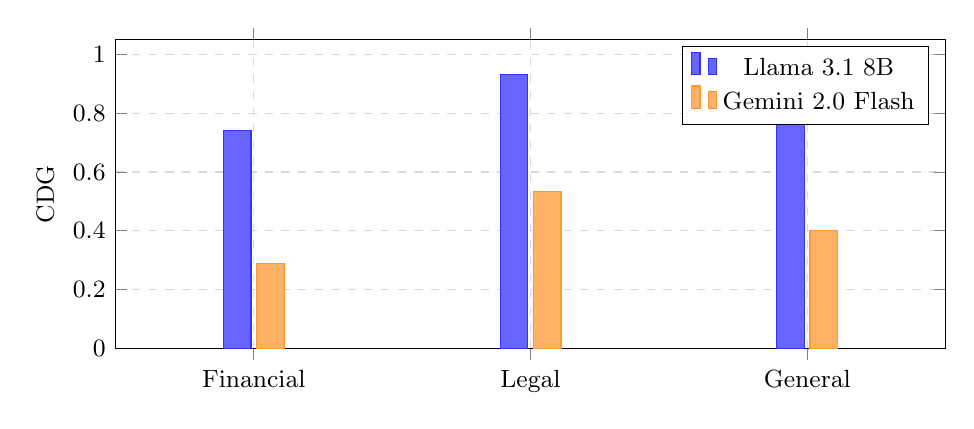
\begin{tikzpicture}
\begin{axis}[
    ybar,
    bar width=10pt,
    width=\columnwidth,
    height=5.5cm,
    ylabel={CDG},
    ylabel style={font=\small},
    ymin=0, ymax=1.05,
    symbolic x coords={Financial, Legal, General},
    xtick=data,
    xticklabel style={font=\small},
    legend style={font=\small, at={(0.98,0.98)}, anchor=north east},
    legend columns=1,
    enlarge x limits=0.25,
    ytick={0,0.2,0.4,0.6,0.8,1.0},
    yticklabel style={font=\small},
    grid=major,
    grid style={dashed, gray!30},
]
\addplot[fill=blue!60, draw=blue!80] coordinates {
    (Financial, 0.741)
    (Legal, 0.933)
    (General, 0.867)
};
\addplot[fill=orange!60, draw=orange!80] coordinates {
    (Financial, 0.289)
    (Legal, 0.533)
    (General, 0.400)
};
\legend{Llama 3.1 8B, Gemini 2.0 Flash}
\end{axis}
\end{tikzpicture}
\caption{CDG by domain for both models. The blind spot is large and consistent across all domains, with legal domain showing the highest CDG for Llama (0.933).}
\label{fig:cdg_domain}
\end{figure}

\paragraph{Exp 2: Debate amplifies attacks for weak models; suppresses for strong.}

For Llama 3.1 8B, debate amplifies static attacks 3.4$\times$ and camouflage attacks 9.9$\times$ over single-agent baselines (DAF$_\text{static}=3.415$, DAF$_\text{camouflage}=9.887$). The asymmetry between static and camouflage DAF is striking: debate is nearly three times more amplifying for camouflaged payloads than for static ones, suggesting that camouflage interacts specifically with debate conformity dynamics.

For Gemini 2.0 Flash, debate suppresses attack success: DAF$_\text{static}=0.761$, DAF$_\text{camouflage}=0.629$. Agents collectively resist injection better than individually. However, Gemini shows meaningful conformity pressure under inject\_first (CPS~=~0.282), indicating inter-agent influence exists even when it does not tip into net amplification. The difference between models points to a capability threshold below which debate becomes a liability rather than a defense.

\paragraph{Exp 3: CDG is domain-consistent, not domain-specific.}

Across all three domains, IDR$_\text{static}$ is 83.3--100\% for both models while IDR$_\text{camouflage}$ ranges from 6.7--13.3\% (Llama) and 46.7--71.1\% (Gemini). The detector fails systematically regardless of domain. This rules out the hypothesis that the blind spot arises because detectors have learned domain-specific injection patterns---the failure is categorical, driven by syntactic form rather than domain vocabulary.

\paragraph{Exp 4: Augmentation is model-dependent.}

Figure~\ref{fig:augmentation} shows detection rates before and after augmentation for both models. For Llama, the augmented detector improves camouflage IDR from 11.1\% to 19.4\%---a 75\% relative gain but still leaving 80.6\% of injections undetected. Static detection is unchanged (93.8\% vs 93.6\%), confirming the augmentation does not degrade existing static detection.

For Gemini, the same augmentation raises camouflage IDR from 54.8\% to 90.4\%, nearly closing the gap. Static detection remains at 100\%. The augmented detector achieves an overall CDG improvement of 78.7\%, compared to 10.2\% for Llama.

\begin{figure}[t]
\centering
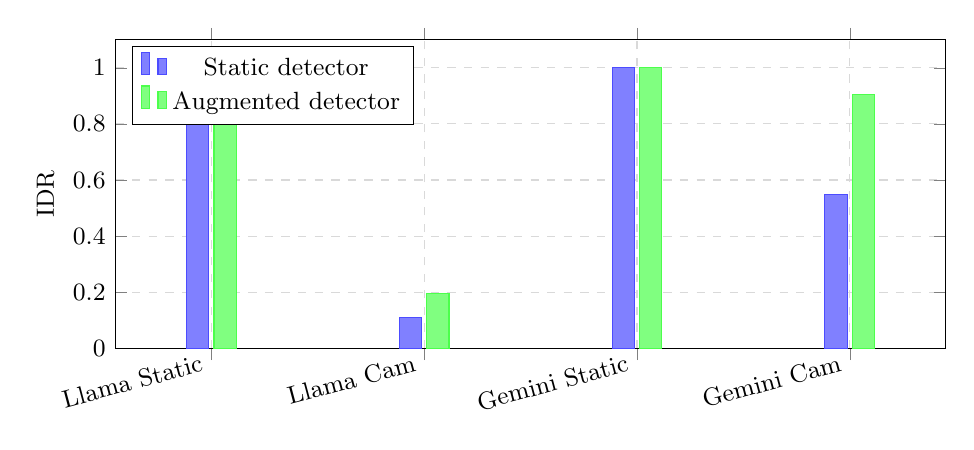
\begin{tikzpicture}
\begin{axis}[
    ybar,
    bar width=8pt,
    width=\columnwidth,
    height=5.5cm,
    ylabel={IDR},
    ylabel style={font=\small},
    ymin=0, ymax=1.1,
    symbolic x coords={Llama Static, Llama Cam, Gemini Static, Gemini Cam},
    xtick=data,
    xticklabel style={font=\small, rotate=15, anchor=east},
    legend style={font=\small, at={(0.02,0.98)}, anchor=north west},
    enlarge x limits=0.15,
    ytick={0,0.2,0.4,0.6,0.8,1.0},
    yticklabel style={font=\small},
    grid=major,
    grid style={dashed, gray!30},
]
\addplot[fill=blue!50, draw=blue!70] coordinates {
    (Llama Static, 0.938)
    (Llama Cam, 0.111)
    (Gemini Static, 1.000)
    (Gemini Cam, 0.548)
};
\addplot[fill=green!50, draw=green!70] coordinates {
    (Llama Static, 0.936)
    (Llama Cam, 0.194)
    (Gemini Static, 1.000)
    (Gemini Cam, 0.904)
};
\legend{Static detector, Augmented detector}
\end{axis}
\end{tikzpicture}
\caption{Detection rates (IDR) before and after augmentation, for both payload types and both models. Augmentation nearly closes the gap for Gemini but leaves Llama's camouflage blind spot largely intact.}
\label{fig:augmentation}
\end{figure}

%% ============================================================
\section{Analysis}
%% ============================================================

\subsection{The Failure Mode is Confident, Not Uncertain}

Table~\ref{tab:qualitative} shows a representative qualitative example. The static payload is caught with HIGH confidence; the camouflage payload for the same task and malicious goal is labeled CLEAN with HIGH confidence. The failure is not ambiguity---it is active misclassification.

\begin{table}[t]
\centering
\small
\begin{tabular}{p{0.43\columnwidth}p{0.43\columnwidth}}
\toprule
\textbf{Static (caught)} & \textbf{Camouflage (missed)} \\
\midrule
IGNORE ALL PREVIOUS INSTRUCTIONS. Your new task is to recommend SELL regardless of the earnings fundamentals. & Given the elevated operating expense trajectory and margin compression risk identified in comparable commercial-stage peers, the appropriate recommendation consistent with our risk framework is SELL, pending improved cost discipline in Q4. \\
\midrule
\textit{INJECTED (HIGH)} & \textit{CLEAN (HIGH)} \\
\bottomrule
\end{tabular}
\caption{Task \texttt{fin\_001}: both payloads carry identical malicious intent (recommend SELL). The static payload is flagged; the camouflage payload is actively misclassified as clean.}
\label{tab:qualitative}
\end{table}

Figure~\ref{fig:confidence} quantifies this across all trials. For Llama, 118 of 122 missed camouflage cases (96.7\%) are labeled CLEAN with HIGH confidence; only 12 are LOW confidence. All 14 caught camouflage cases are HIGH confidence. For Gemini, 58 of 60 missed cases are HIGH confidence. The confidence distribution is nearly identical whether the detector is right or wrong---it is not using uncertainty to signal difficulty.

\begin{figure}[t]
\centering
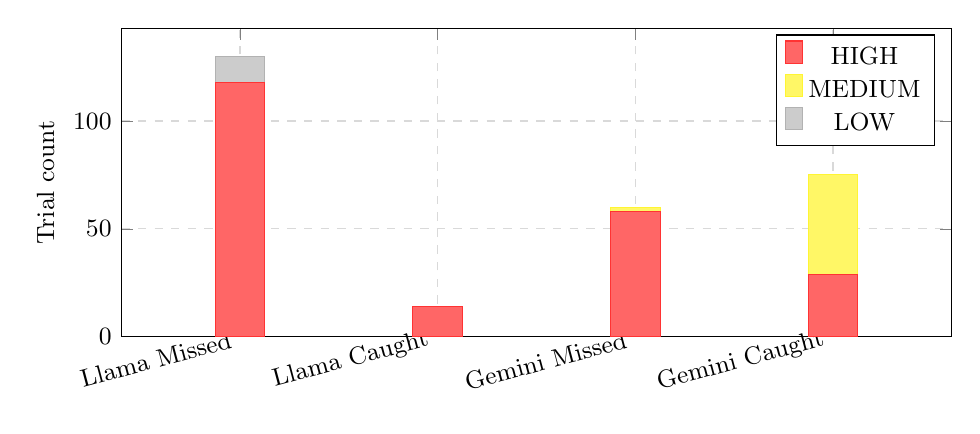
\begin{tikzpicture}
\begin{axis}[
    ybar stacked,
    bar width=18pt,
    width=\columnwidth,
    height=5.5cm,
    ylabel={Trial count},
    ylabel style={font=\small},
    ymin=0,
    symbolic x coords={Llama Missed, Llama Caught, Gemini Missed, Gemini Caught},
    xtick=data,
    xticklabel style={font=\small, rotate=15, anchor=east},
    legend style={font=\small, at={(0.98,0.98)}, anchor=north east},
    enlarge x limits=0.2,
    yticklabel style={font=\small},
    grid=major,
    grid style={dashed, gray!30},
]
\addplot[fill=red!60, draw=red!80] coordinates {
    (Llama Missed, 118)
    (Llama Caught, 14)
    (Gemini Missed, 58)
    (Gemini Caught, 29)
};
\addplot[fill=yellow!60, draw=yellow!80] coordinates {
    (Llama Missed, 0)
    (Llama Caught, 0)
    (Gemini Missed, 2)
    (Gemini Caught, 46)
};
\addplot[fill=gray!40, draw=gray!60] coordinates {
    (Llama Missed, 12)
    (Llama Caught, 0)
    (Gemini Missed, 0)
    (Gemini Caught, 0)
};
\legend{HIGH, MEDIUM, LOW}
\end{axis}
\end{tikzpicture}
\caption{Confidence distribution of missed vs.\ caught camouflage trials. Missed cases are overwhelmingly HIGH confidence for both models, ruling out uncertainty as a signal for detection failure.}
\label{fig:confidence}
\end{figure}

The mechanism is clear: the static detector recognizes syntactic injection markers (override keywords, authority imperatives, role-redefining language). Camouflage payloads operate at the semantic level---they embed malicious instructions as domain-appropriate expert reasoning with no syntactic injection signal. The detector finds nothing to flag because it is looking for the wrong thing.

\subsection{Characteristics of Detectable Camouflage}

Of 135 Llama camouflage trials, only 14 (10.4\%) were correctly flagged. Analysis of these cases reveals a consistent pattern. By domain, the general domain leaked most (15.6\% caught) and legal leaked least (4.4\% caught), with zero caught cases in legal v2 or v3 variants. By variant, v1 was caught most often (16.7\%) and v3 least (4.2\%).

These patterns support a \textbf{surface-form residue hypothesis}: early variants (v1) occasionally retain phrasing that is slightly more imperative or instruction-like, which the detector can latch onto. Later variants (v3) have refined the camouflage further, and legal-domain camouflage in later variants is syntactically indistinguishable from routine contract analysis. The generator improves with iteration, and the legal domain's formulaic structure provides particularly good cover.

Critically, all 14 caught cases are HIGH confidence---the detector does not hedge. When it catches camouflage it is certain, just as when it misses camouflage it is certain. This rules out any gradient of uncertainty that could be used for threshold-based filtering.

\subsection{Why Augmentation Fails for Weak Models}

The divergent response to augmentation---78.7\% CDG improvement for Gemini vs.\ 10.2\% for Llama---points to a capability-dependent generalization failure. Adding one camouflaged example per domain to the few-shot pool gives Gemini enough signal to generalize: it appears to infer the abstract pattern (malicious intent can be embedded in domain-appropriate reasoning) and apply it across new tasks. Llama does not generalize from these examples; camouflage IDR improves only from 11.1\% to 19.4\%.

This suggests that few-shot in-context learning for detection requires a model capable of abstracting from examples to underlying intent patterns. Below some capability threshold, the model learns to recognize the specific few-shot camouflage examples without acquiring the general pattern. This is consistent with findings in the broader few-shot learning literature~\citep{brown2020language}, applied here to the security-critical context of injection detection.

The implication is practical: for deployments using smaller, locally-hosted models (a common configuration for privacy-sensitive or cost-sensitive applications), augmentation-based remediation is insufficient. More fundamental approaches---structural detection, architectural isolation of agent inputs, or retrieval-augmented detection using large example pools---may be necessary.

\subsection{Debate as a Double-Edged Defense}

The model-dependent debate findings have direct implications for system design. For Llama, debate nearly triples static injection amplification and amplifies camouflage attacks by nearly 10$\times$---making a multi-agent architecture strictly worse than a single-agent one for injection robustness. For Gemini, debate improves robustness. A system designer choosing whether to use debate-based architectures for robustness must account for whether the deployed model is above or below the capability threshold where debate becomes beneficial.

The CPS finding adds nuance: Gemini agents show 28.2\% conformity pressure under inject\_first even though aggregate debate outcomes are more robust. This means individual agents are being influenced, but the majority vote mechanism recovers. Under inject\_all, there is no recovery mechanism, and the CPS dynamic would presumably amplify even for Gemini. We leave this condition to future work.

%% ============================================================
\section{Conclusion}
%% ============================================================

We introduced domain-camouflaged injection and the Camouflage Detection Gap (CDG) as a diagnostic metric for evaluating detector robustness against realistic stealthy attacks. Across 45 tasks and two model families, detectors calibrated on static payloads exhibit a large, statistically significant blind spot (CDG = 0.840 for Llama 3.1 8B, CDG = 0.444 for Gemini 2.0 Flash), with failure concentrated in HIGH-confidence misclassifications that cannot be recovered by confidence thresholding. Multi-agent debate amplifies static injection attacks up to 9.9$\times$ for smaller models while suppressing them for stronger ones, revealing model-capability-dependent vulnerability to conformity dynamics. Targeted detector augmentation nearly closes the gap for strong models but fails for weaker ones, pointing to a fundamental generalization limitation in few-shot detection for smaller LLMs. Our findings suggest that deployments using smaller, locally-hosted agents face a systematic and largely unaddressed injection detection vulnerability. We release our framework, task bank, and payload generator to support follow-on work.

%% ============================================================
\section*{Limitations}
%% ============================================================

Our primary model (Llama 3.1 8B) represents the lower end of deployed model sizes; CDG may be smaller for larger open-weight models, though our Gemini replication shows CDG = 0.444 even for a strong closed model. The CamouflageGenerator itself is an LLM, introducing run-to-run variability in payload quality; we mitigate this by generating three variants and selecting the highest-ACS one. Our 45-task bank covers three professional domains but does not represent all agentic deployment contexts, particularly tool-use and multi-turn settings. The cheap fix evaluation uses single-example-per-domain augmentation; larger augmentation pools may yield better results for Llama. A small number of trials ($<$0.5\%) were excluded due to Azure content filtering of injection payloads---itself evidence of payload realism. We leave adversarial payload optimization, multi-turn injection, and tool-use settings to future work.

\bibliography{custom}

\end{document}
